\section{Kiểm chứng tính nhất quán của hệ thống}
\label{sec:kiem_chung_nhat_quan}

Khi triển khai các hệ thống học máy tại biên, hiện tượng không khớp triển khai — sự sai lệch kết quả suy luận giữa môi trường huấn luyện (Python/TensorFlow) và môi trường thực thi (C++/TFLite Micro) — là vấn đề phổ biến. Phần này trình bày các phương pháp kiểm chứng tính nhất quán của toàn bộ đường ống xử lý, từ tiền xử lý đến suy luận cuối cùng.

\subsection{Đối chiếu phân phối đặc trưng giữa môi trường giả lập và phần cứng}

Trong giai đoạn đầu phát triển, mô hình đạt độ chính xác cao trên tập kiểm thử nhưng sinh ra nhiều cảnh báo giả khi nạp xuống vi điều khiển Seeed Studio XIAO ESP32-S3. Nguyên nhân bắt nguồn từ sự bất đồng bộ trong thuật toán trích xuất đặc trưng âm thanh giữa hai môi trường.

Kịch bản Python ban đầu sử dụng thư viện \texttt{librosa} với độ chính xác kép (Float64), trong khi firmware C++ sử dụng thư viện \texttt{esp-dsp} với Float32. Sự khác biệt về thư viện và độ chính xác số học này làm thay đổi phân phối dữ liệu đầu vào.

Để khắc phục, hệ thống thực hiện đồng bộ hóa thuật toán:
\begin{itemize}
    \item \textbf{Đồng nhất tham số DSP:} Loại bỏ sự phụ thuộc vào \texttt{librosa}. Mã nguồn Python được viết lại bằng NumPy để mô phỏng logic tính toán của vi điều khiển. Cấu hình cố định: cửa sổ Hann, FFT 512 điểm và bước trượt 256 mẫu. Với bộ đệm 1 giây ở tần số lấy mẫu 8 kHz, số khung hợp lệ được tính theo $\lfloor(8000-512)/256\rfloor + 1 = 30$, đúng với cấu hình firmware.
    \item \textbf{Cố định dải động:} Năng lượng tín hiệu qua bộ lọc Mel được giới hạn và ánh xạ về khoảng $[-80, 0]$ dB trên cả hai môi trường. Xác thực thông qua đồ thị phân phối xác minh ma trận đặc trưng từ Python và dữ liệu từ bộ nhớ của vi điều khiển Seeed Studio XIAO ESP32-S3 trùng khớp ở cấp độ bit.
\end{itemize}

\begin{figure}[H]
    \centering
    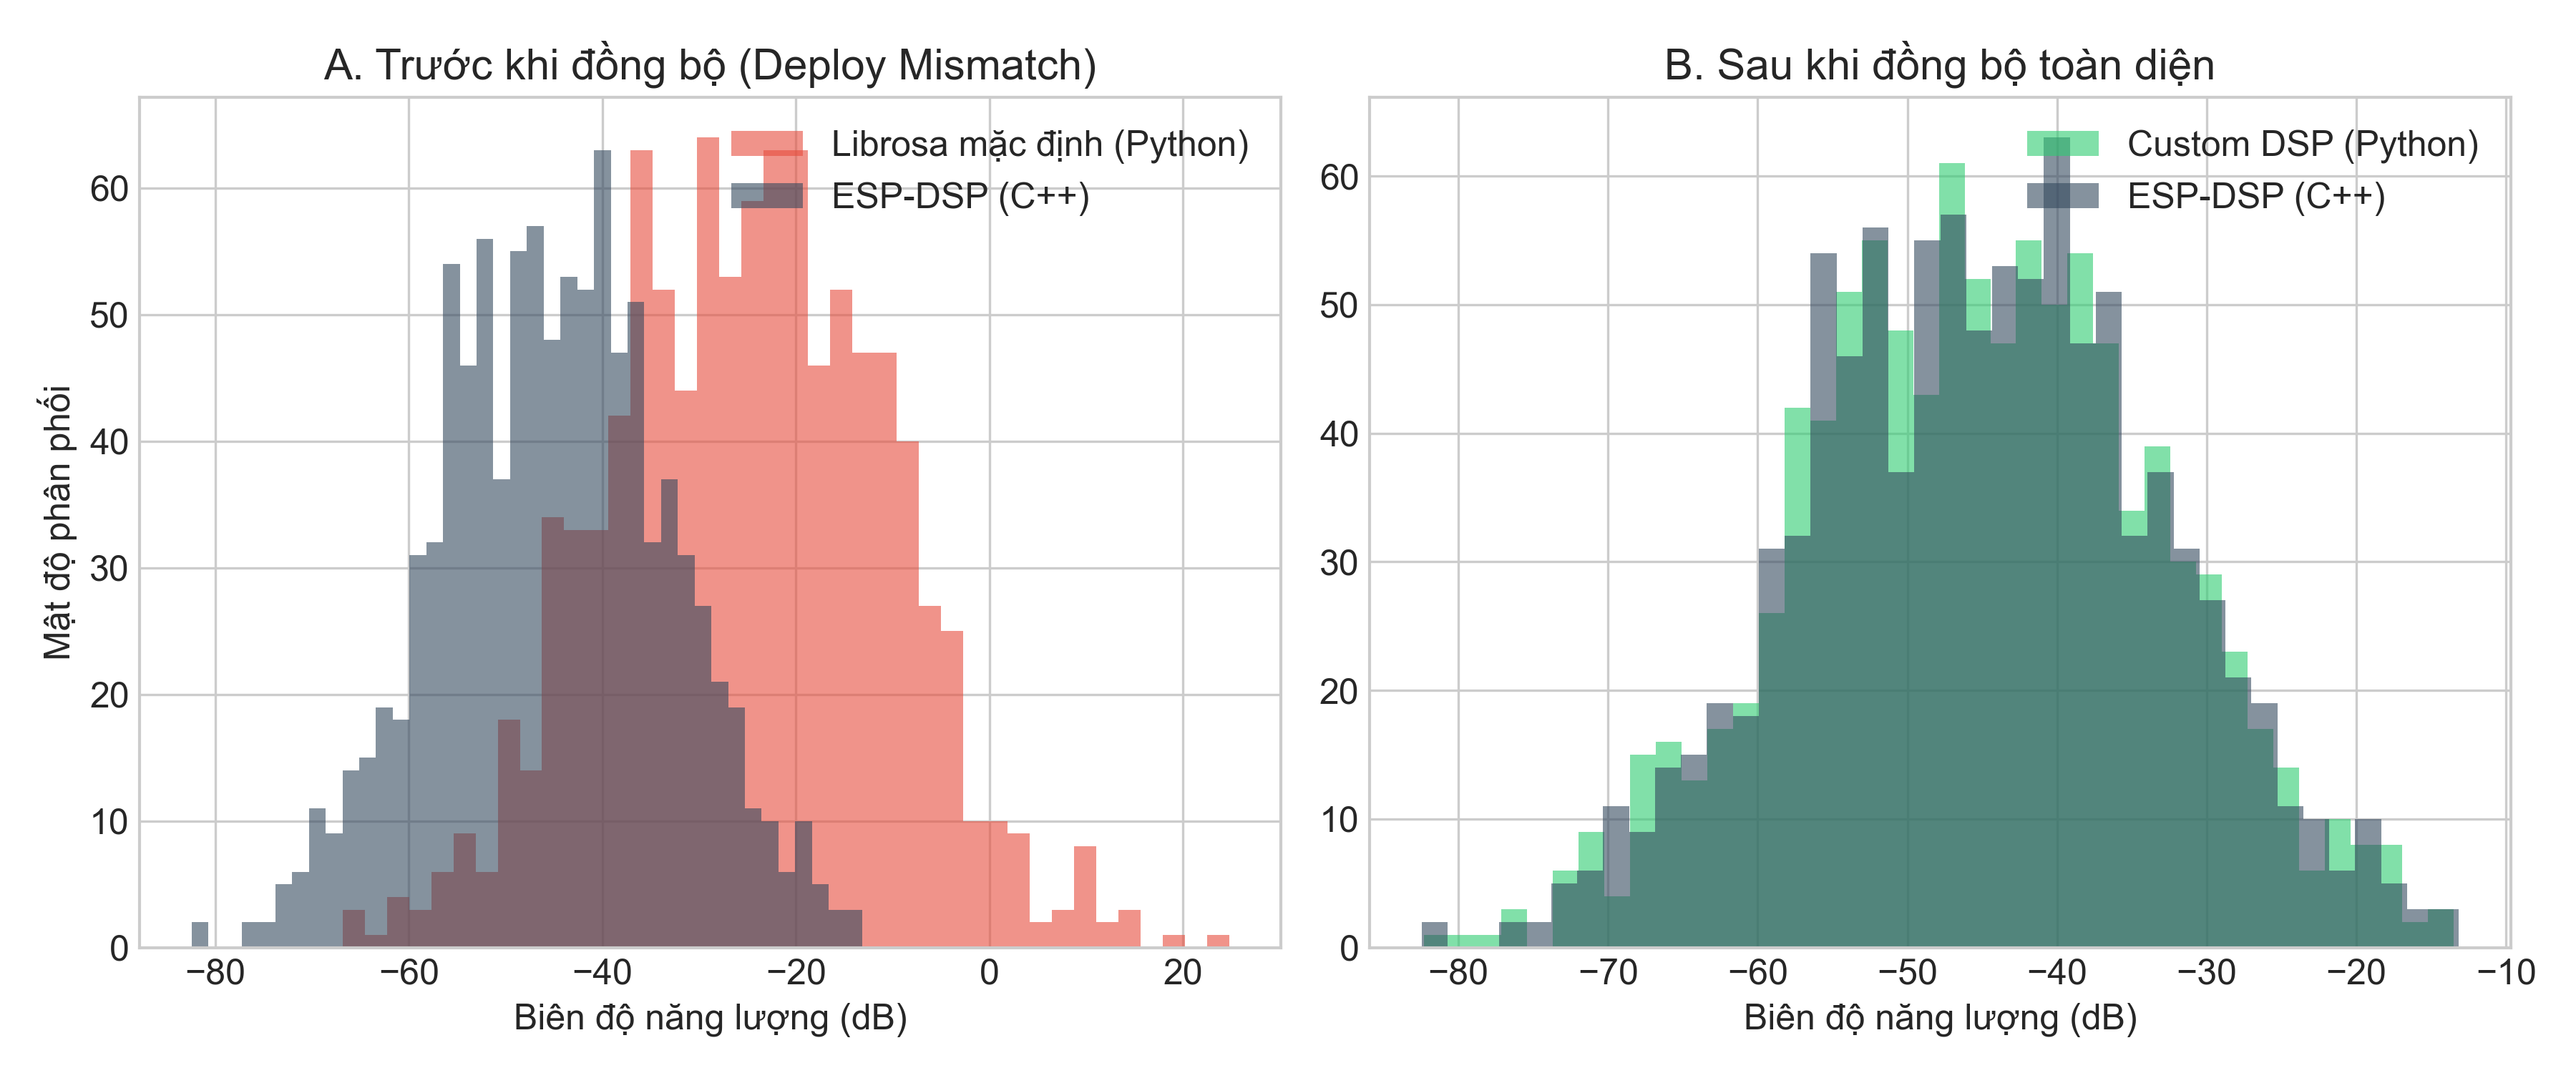
\includegraphics[width=0.9\linewidth]{chap4/image/dsp_histogram_match.png}
    \caption[Đối chiếu phân phối năng lượng âm thanh]{Đối chiếu phân phối năng lượng phổ âm thanh trước và sau khi đồng bộ thuật toán DSP giữa Python và C++.}
    \label{fig:dsp_mismatch}
\end{figure}

\subsection{Xác thực tính toàn vẹn của đồ thị suy luận}

Sau khi xuất mô hình dưới dạng mảng byte, xác thực tính toàn vẹn bộ nhớ khi nạp qua TensorFlow Lite Micro là bước quan trọng. Hệ thống sử dụng xác thực chéo ở cấp độ tensor:

\begin{enumerate}
    \item \textbf{Trích xuất vector kiểm thử:} 100 vector đặc trưng ngẫu nhiên từ Python được sử dụng làm dữ liệu nền kiểm chứng.
    \item \textbf{Quản lý vùng nhớ an toàn:} Để tránh lỗi phân mảnh và tràn bộ nhớ cấp phát động, mảng bộ nhớ làm việc trung gian (\texttt{tensor\_arena}) được cấp phát tĩnh. Kích thước vùng nhớ được tính toán tối ưu với cấu trúc mạng và đặt tại phân vùng SRAM nội bộ để tăng tốc độ truy xuất. Điều này cho phép thiết bị chuyển đổi linh hoạt giữa 3 mô hình (GENTLE, STRONG, SPIN) trên cùng một vùng nhớ trung gian mà không cần cấp phát lại bộ nhớ.
    \item \textbf{Suy luận song song và đối chiếu:} Một vector đầu vào được đưa qua mô hình Float32 trên máy tính và mô hình INT8 trên vi điều khiển. Đầu ra \texttt{int8\_t} từ vi điều khiển Seeed Studio XIAO ESP32-S3 được gửi qua cổng Serial để so sánh từng phần tử với mảng đầu ra trên máy chủ.
\end{enumerate}

Bộ thông dịch TFLM thực thi đồ thị mạng ổn định, không ghi nhận tràn vùng nhớ đệm hay lỗi sai số vượt ngưỡng trong quá trình lượng tử hóa.
